% =====================================================================
% RASCUNHO -- diagrama do BCD-MMSE com a inicialização BDAC-MMSE, MODELO B
% (covariância estimada em cada PRB, como na Seção VI do artigo, L577).
% O modelo A está em rascunho_diagrama_bcd_modelo_a.tex.
% ---------------------------------------------------------------------
% Mesmo estilo da Figura fig:fluxo_m7 (rascunho_diagrama_equalizadores).
% Visão de uma DU genérica c na cadeia: à esquerda a DU anterior, à
% direita a próxima. Caixas laranja = passos com inversão de matriz.
%
% Conferido em referencias/zhao2025_jsac/paper.md:
%   inicialização BDAC, Eq. (7) ............... L136-L142
%   Algoritmo 3 (pré-processamento de A e b) .. L407-L436
%   atualização W_c^l, Eq. (30) ............... L504
%   atualização de A e b, Eqs. (28)-(29) ...... L443-L449
%   anel: DU anterior à DU 1 é a DU C ......... nota 6, L459
%   filtro: soma de W_c y_c pela cadeia ....... L430-L434, Fig. 5(b)
% Escolhas da autora (não estão no artigo):
%   - G_c^{-1} é invertida uma vez por PRB e reutilizada nas T iterações
%     (no Algoritmo 3 ela fica dentro do laço);
%   - a soma K x K da inicialização é acumulada pelo anel e invertida na
%     DU C (o artigo só diz "in a decentralized manner", L410);
%   - Phi_c é nome local para a soma acumulada.
% =====================================================================

\usetikzlibrary{positioning, fit, backgrounds, calc}

\begin{figure}[htbp]
\caption{BCD-MMSE com inicialização BDAC-MMSE, modelo B (covariância estimada em
cada PRB): passos em uma DU $c$ e dados trocados com as DUs vizinhas.}
\label{fig:fluxo_bcd_b}
\centering
\footnotesize
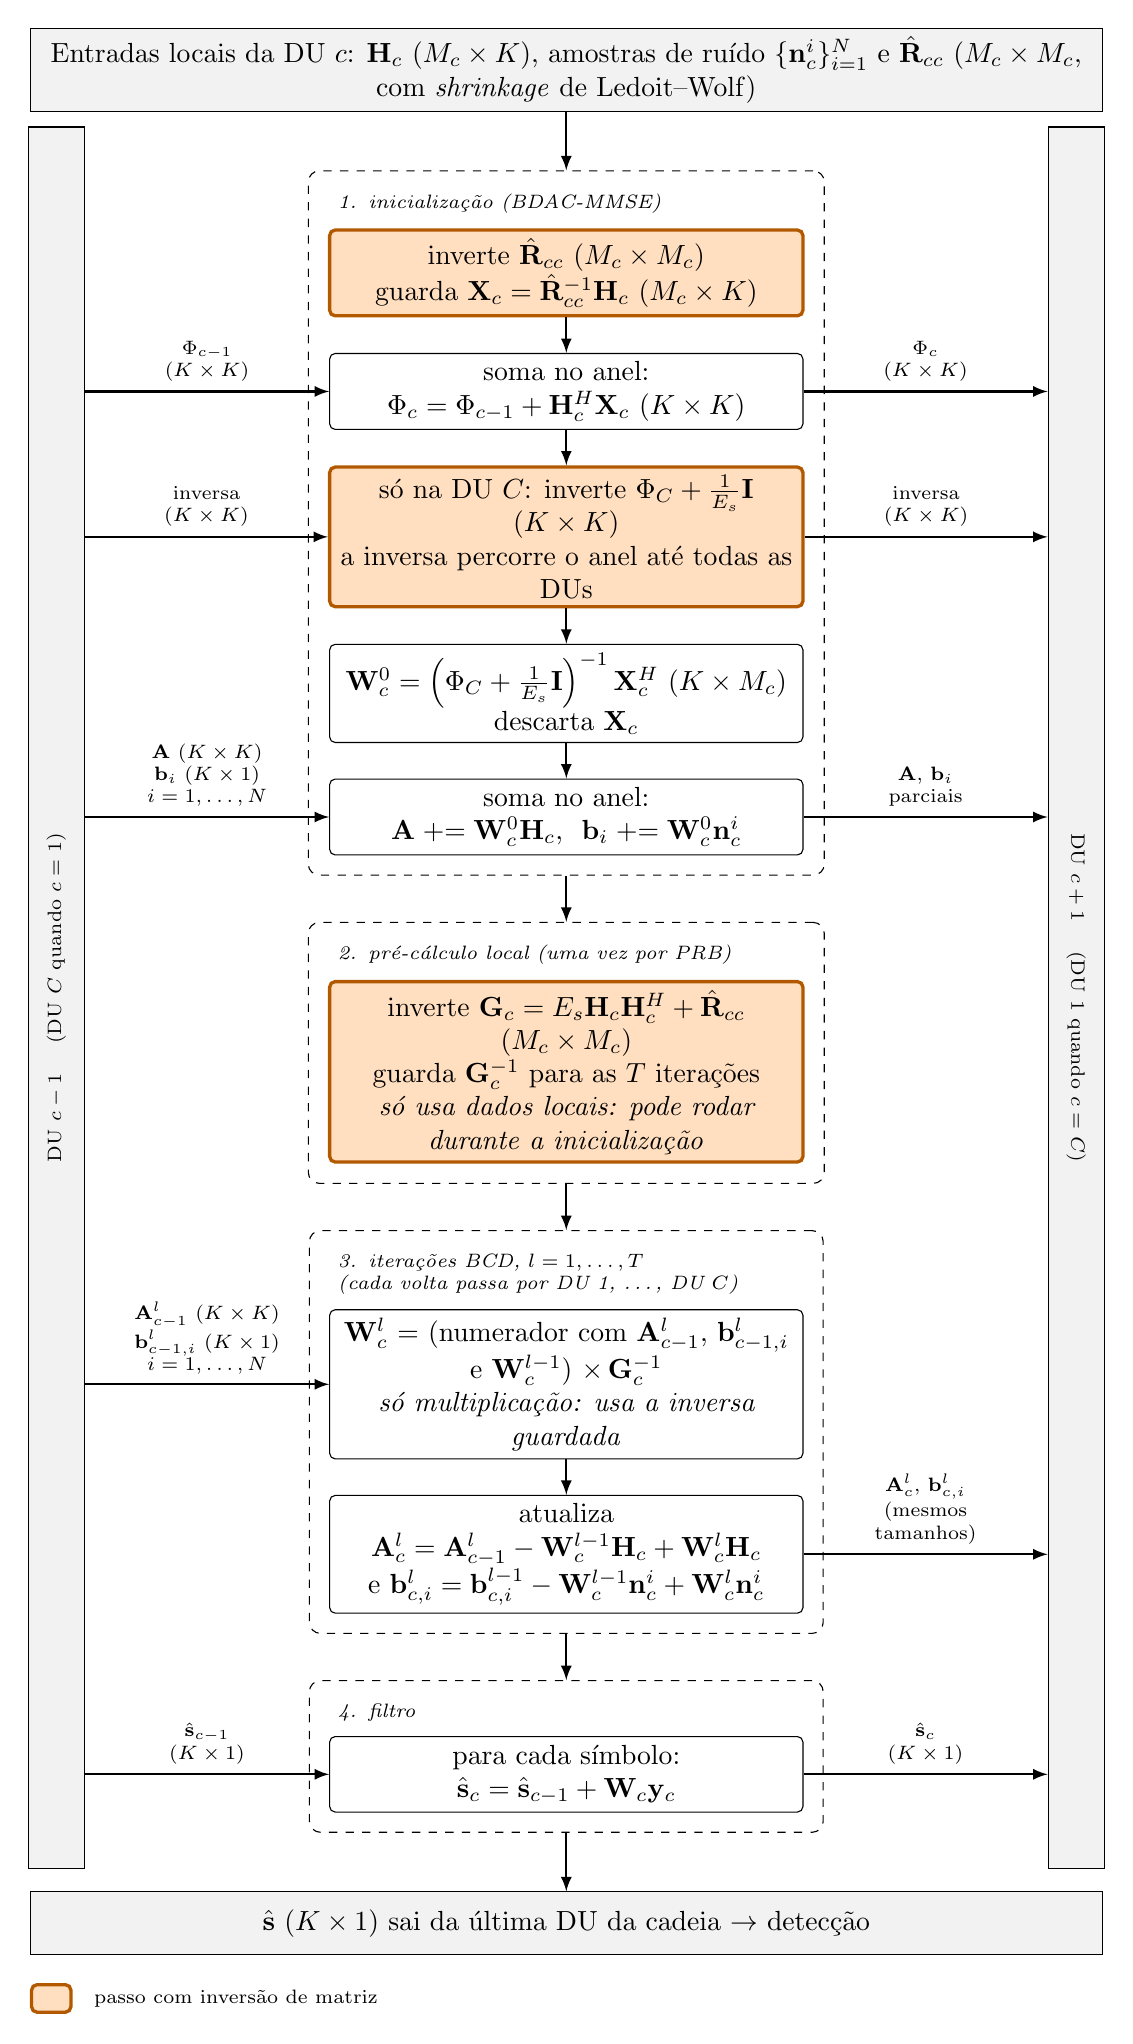
\begin{tikzpicture}[
    node distance = 0.45cm and 0.35cm,
    caixa/.style = {draw, rounded corners=2pt, align=flush center, fill=white,
                     minimum height=0.9cm, inner sep=3pt, text width=5.8cm},
    inv/.style   = {caixa, fill=orange!25, draw=orange!70!black, very thick},
    dado/.style  = {draw, align=flush center, fill=gray!10, minimum height=0.8cm,
                     inner sep=3pt},
    grupo/.style = {draw, dashed, rounded corners=4pt, inner sep=0.25cm},
    seta/.style  = {-latex, thick},
    rot/.style   = {font=\scriptsize, align=center, above},
    titulo/.style = {font=\scriptsize\itshape, align=left, text width=5.8cm,
                     inner sep=1pt},
  ]

  % --- entradas -----------------------------------------------------------
  \node[dado, text width=13.4cm] (in) {Entradas locais da DU $c$:
    $\mathbf{H}_c$ ($M_c \times K$), amostras de ruído
    $\{\mathbf{n}_c^i\}_{i=1}^{N}$ e $\hat{\mathbf{R}}_{cc}$ ($M_c \times M_c$,
    com \textit{shrinkage} de Ledoit--Wolf)};

  % --- 1. inicialização (BDAC-MMSE) --------------------------------------
  \node[titulo, below=1.0cm of in] (t1) {1. inicialização (BDAC-MMSE)};
  \node[inv, below=0.15cm of t1] (rcc) {inverte $\hat{\mathbf{R}}_{cc}$
    ($M_c \times M_c$)\\
    guarda $\mathbf{X}_c = \hat{\mathbf{R}}_{cc}^{-1}\mathbf{H}_c$ ($M_c \times K$)};
  \node[caixa, below=of rcc] (phi) {soma no anel:\\
    $\boldsymbol{\Phi}_c = \boldsymbol{\Phi}_{c-1} + \mathbf{H}_c^H\mathbf{X}_c$
    ($K \times K$)};
  \node[inv, below=of phi] (kk) {só na DU $C$: inverte
    $\boldsymbol{\Phi}_C + \frac{1}{E_s}\mathbf{I}$ ($K \times K$)\\
    a inversa percorre o anel até todas as DUs};
  \node[caixa, below=of kk] (w0) {$\mathbf{W}_c^0 =
    \left(\boldsymbol{\Phi}_C + \frac{1}{E_s}\mathbf{I}\right)^{-1}\mathbf{X}_c^H$
    ($K \times M_c$)\\ descarta $\mathbf{X}_c$};
  \node[caixa, below=of w0] (ab0) {soma no anel:\\
    $\mathbf{A} \mathrel{+}= \mathbf{W}_c^0\mathbf{H}_c$, \
    $\mathbf{b}_i \mathrel{+}= \mathbf{W}_c^0\mathbf{n}_c^i$};

  % --- 2. pré-cálculo local ----------------------------------------------
  \node[titulo, below=1.1cm of ab0] (t2) {2. pré-cálculo local (uma vez por PRB)};
  \node[inv, below=0.15cm of t2] (gc) {inverte
    $\mathbf{G}_c = E_s\mathbf{H}_c\mathbf{H}_c^H + \hat{\mathbf{R}}_{cc}$
    ($M_c \times M_c$)\\
    guarda $\mathbf{G}_c^{-1}$ para as $T$ iterações\\
    \textit{só usa dados locais: pode rodar durante a inicialização}};

  % --- 3. iterações BCD ---------------------------------------------------
  \node[titulo, below=1.1cm of gc] (t3) {3. iterações BCD, $l = 1, \dots, T$\\
    (cada volta passa por DU 1, \dots, DU $C$)};
  \node[caixa, below=0.15cm of t3] (wl) {$\mathbf{W}_c^l$ = (numerador com
    $\mathbf{A}_{c-1}^l$, $\mathbf{b}_{c-1,i}^l$ e $\mathbf{W}_c^{l-1}$)
    $\times\, \mathbf{G}_c^{-1}$\\
    \textit{só multiplicação: usa a inversa guardada}};
  \node[caixa, below=of wl] (abl) {atualiza
    $\mathbf{A}_c^l = \mathbf{A}_{c-1}^l - \mathbf{W}_c^{l-1}\mathbf{H}_c
    + \mathbf{W}_c^l\mathbf{H}_c$\\
    e $\mathbf{b}_{c,i}^l = \mathbf{b}_{c,i}^{l-1}
    - \mathbf{W}_c^{l-1}\mathbf{n}_c^i + \mathbf{W}_c^l\mathbf{n}_c^i$};

  % --- 4. filtro ----------------------------------------------------------
  \node[titulo, below=1.1cm of abl] (t4) {4. filtro};
  \node[caixa, below=0.15cm of t4] (filt) {para cada símbolo:\\
    $\hat{\mathbf{s}}_c = \hat{\mathbf{s}}_{c-1} + \mathbf{W}_c\mathbf{y}_c$};

  % --- saída --------------------------------------------------------------
  \node[dado, text width=13.4cm, below=1.0cm of filt] (out)
    {$\hat{\mathbf{s}}$ ($K \times 1$) sai da última DU da cadeia
    $\rightarrow$ detecção};

  % --- grupos -------------------------------------------------------------
  \begin{scope}[on background layer]
    \node[grupo, fit=(t1) (rcc) (ab0)] (g1) {};
    \node[grupo, fit=(t2) (gc)] (g2) {};
    \node[grupo, fit=(t3) (wl) (abl)] (g3) {};
    \node[grupo, fit=(t4) (filt)] (g4) {};
  \end{scope}

  % --- DUs vizinhas (linhas de vida) --------------------------------------
  \coordinate (Ltop) at ($(g1.north west) + (-3.2cm, 0.2cm)$);
  \coordinate (Lbot) at ($(g4.south west) + (-3.2cm, -0.1cm)$);
  \coordinate (Rtop) at ($(g1.north east) + (3.2cm, 0.2cm)$);
  \coordinate (Rbot) at ($(g4.south east) + (3.2cm, -0.1cm)$);
  \node[dado, fit=(Ltop) (Lbot), inner sep=0.35cm] (L) {};
  \node[dado, fit=(Rtop) (Rbot), inner sep=0.35cm] (R) {};
  \node[rotate=90, font=\scriptsize, align=center] at (L.center)
    {DU $c-1$ \quad (DU $C$ quando $c = 1$)};
  \node[rotate=270, font=\scriptsize, align=center] at (R.center)
    {DU $c+1$ \quad (DU $1$ quando $c = C$)};

  % --- setas: fluxo interno -----------------------------------------------
  \draw[seta] (in) -- (g1.north);
  \draw[seta] (rcc) -- (phi);
  \draw[seta] (phi) -- (kk);
  \draw[seta] (kk) -- (w0);
  \draw[seta] (w0) -- (ab0);
  \draw[seta] (g1) -- (g2);
  \draw[seta] (g2) -- (g3);
  \draw[seta] (wl) -- (abl);
  \draw[seta] (g3) -- (g4);
  \draw[seta] (g4) -- (out);

  % --- setas: dados trocados com as DUs vizinhas --------------------------
  \draw[seta] (L.east |- phi) -- node[rot] {$\boldsymbol{\Phi}_{c-1}$\\($K \times K$)} (phi);
  \draw[seta] (phi) -- node[rot] {$\boldsymbol{\Phi}_c$\\($K \times K$)} (R.west |- phi);
  \draw[seta] (L.east |- kk) -- node[rot] {inversa\\($K \times K$)} (kk);
  \draw[seta] (kk) -- node[rot] {inversa\\($K \times K$)} (R.west |- kk);
  \draw[seta] (L.east |- ab0) -- node[rot] {$\mathbf{A}$ ($K \times K$)\\
    $\mathbf{b}_i$ ($K \times 1$)\\ $i = 1, \dots, N$} (ab0);
  \draw[seta] (ab0) -- node[rot] {$\mathbf{A}$, $\mathbf{b}_i$\\parciais} (R.west |- ab0);
  \draw[seta] (L.east |- wl) -- node[rot] {$\mathbf{A}_{c-1}^l$ ($K \times K$)\\
    $\mathbf{b}_{c-1,i}^l$ ($K \times 1$)\\ $i = 1, \dots, N$} (wl);
  \draw[seta] (abl) -- node[rot] {$\mathbf{A}_c^l$, $\mathbf{b}_{c,i}^l$\\
    (mesmos\\tamanhos)} (R.west |- abl);
  \draw[seta] (L.east |- filt) -- node[rot] {$\hat{\mathbf{s}}_{c-1}$\\($K \times 1$)} (filt);
  \draw[seta] (filt) -- node[rot] {$\hat{\mathbf{s}}_c$\\($K \times 1$)} (R.west |- filt);

  % --- legenda ------------------------------------------------------------
  \node[inv, text width={}, minimum height=0.35cm, minimum width=0.5cm, inner sep=0pt,
        below=0.35cm of out.south west, anchor=north west] (leg) {};
  \node[right=0.15cm of leg, font=\scriptsize] {passo com inversão de matriz};
\end{tikzpicture}
\legend{Fonte: a autora, com base em \citeonline{zhao2025jsac}.}
\end{figure}
